% Options for packages loaded elsewhere
\PassOptionsToPackage{unicode}{hyperref}
\PassOptionsToPackage{hyphens}{url}
%
\documentclass[
  man]{apa6}
\usepackage{amsmath,amssymb}
\usepackage{iftex}
\ifPDFTeX
  \usepackage[T1]{fontenc}
  \usepackage[utf8]{inputenc}
  \usepackage{textcomp} % provide euro and other symbols
\else % if luatex or xetex
  \usepackage{unicode-math} % this also loads fontspec
  \defaultfontfeatures{Scale=MatchLowercase}
  \defaultfontfeatures[\rmfamily]{Ligatures=TeX,Scale=1}
\fi
\usepackage{lmodern}
\ifPDFTeX\else
  % xetex/luatex font selection
\fi
% Use upquote if available, for straight quotes in verbatim environments
\IfFileExists{upquote.sty}{\usepackage{upquote}}{}
\IfFileExists{microtype.sty}{% use microtype if available
  \usepackage[]{microtype}
  \UseMicrotypeSet[protrusion]{basicmath} % disable protrusion for tt fonts
}{}
\makeatletter
\@ifundefined{KOMAClassName}{% if non-KOMA class
  \IfFileExists{parskip.sty}{%
    \usepackage{parskip}
  }{% else
    \setlength{\parindent}{0pt}
    \setlength{\parskip}{6pt plus 2pt minus 1pt}}
}{% if KOMA class
  \KOMAoptions{parskip=half}}
\makeatother
\usepackage{xcolor}
\usepackage{graphicx}
\makeatletter
\def\maxwidth{\ifdim\Gin@nat@width>\linewidth\linewidth\else\Gin@nat@width\fi}
\def\maxheight{\ifdim\Gin@nat@height>\textheight\textheight\else\Gin@nat@height\fi}
\makeatother
% Scale images if necessary, so that they will not overflow the page
% margins by default, and it is still possible to overwrite the defaults
% using explicit options in \includegraphics[width, height, ...]{}
\setkeys{Gin}{width=\maxwidth,height=\maxheight,keepaspectratio}
% Set default figure placement to htbp
\makeatletter
\def\fps@figure{htbp}
\makeatother
\setlength{\emergencystretch}{3em} % prevent overfull lines
\providecommand{\tightlist}{%
  \setlength{\itemsep}{0pt}\setlength{\parskip}{0pt}}
\setcounter{secnumdepth}{-\maxdimen} % remove section numbering
% Make \paragraph and \subparagraph free-standing
\ifx\paragraph\undefined\else
  \let\oldparagraph\paragraph
  \renewcommand{\paragraph}[1]{\oldparagraph{#1}\mbox{}}
\fi
\ifx\subparagraph\undefined\else
  \let\oldsubparagraph\subparagraph
  \renewcommand{\subparagraph}[1]{\oldsubparagraph{#1}\mbox{}}
\fi
\newlength{\cslhangindent}
\setlength{\cslhangindent}{1.5em}
\newlength{\csllabelwidth}
\setlength{\csllabelwidth}{3em}
\newlength{\cslentryspacingunit} % times entry-spacing
\setlength{\cslentryspacingunit}{\parskip}
\newenvironment{CSLReferences}[2] % #1 hanging-ident, #2 entry spacing
 {% don't indent paragraphs
  \setlength{\parindent}{0pt}
  % turn on hanging indent if param 1 is 1
  \ifodd #1
  \let\oldpar\par
  \def\par{\hangindent=\cslhangindent\oldpar}
  \fi
  % set entry spacing
  \setlength{\parskip}{#2\cslentryspacingunit}
 }%
 {}
\usepackage{calc}
\newcommand{\CSLBlock}[1]{#1\hfill\break}
\newcommand{\CSLLeftMargin}[1]{\parbox[t]{\csllabelwidth}{#1}}
\newcommand{\CSLRightInline}[1]{\parbox[t]{\linewidth - \csllabelwidth}{#1}\break}
\newcommand{\CSLIndent}[1]{\hspace{\cslhangindent}#1}
\ifLuaTeX
\usepackage[bidi=basic]{babel}
\else
\usepackage[bidi=default]{babel}
\fi
\babelprovide[main,import]{english}
% get rid of language-specific shorthands (see #6817):
\let\LanguageShortHands\languageshorthands
\def\languageshorthands#1{}
% Manuscript styling
\usepackage{upgreek}
\captionsetup{font=singlespacing,justification=justified}

% Table formatting
\usepackage{longtable}
\usepackage{lscape}
% \usepackage[counterclockwise]{rotating}   % Landscape page setup for large tables
\usepackage{multirow}		% Table styling
\usepackage{tabularx}		% Control Column width
\usepackage[flushleft]{threeparttable}	% Allows for three part tables with a specified notes section
\usepackage{threeparttablex}            % Lets threeparttable work with longtable

% Create new environments so endfloat can handle them
% \newenvironment{ltable}
%   {\begin{landscape}\centering\begin{threeparttable}}
%   {\end{threeparttable}\end{landscape}}
\newenvironment{lltable}{\begin{landscape}\centering\begin{ThreePartTable}}{\end{ThreePartTable}\end{landscape}}

% Enables adjusting longtable caption width to table width
% Solution found at http://golatex.de/longtable-mit-caption-so-breit-wie-die-tabelle-t15767.html
\makeatletter
\newcommand\LastLTentrywidth{1em}
\newlength\longtablewidth
\setlength{\longtablewidth}{1in}
\newcommand{\getlongtablewidth}{\begingroup \ifcsname LT@\roman{LT@tables}\endcsname \global\longtablewidth=0pt \renewcommand{\LT@entry}[2]{\global\advance\longtablewidth by ##2\relax\gdef\LastLTentrywidth{##2}}\@nameuse{LT@\roman{LT@tables}} \fi \endgroup}

% \setlength{\parindent}{0.5in}
% \setlength{\parskip}{0pt plus 0pt minus 0pt}

% Overwrite redefinition of paragraph and subparagraph by the default LaTeX template
% See https://github.com/crsh/papaja/issues/292
\makeatletter
\renewcommand{\paragraph}{\@startsection{paragraph}{4}{\parindent}%
  {0\baselineskip \@plus 0.2ex \@minus 0.2ex}%
  {-1em}%
  {\normalfont\normalsize\bfseries\itshape\typesectitle}}

\renewcommand{\subparagraph}[1]{\@startsection{subparagraph}{5}{1em}%
  {0\baselineskip \@plus 0.2ex \@minus 0.2ex}%
  {-\z@\relax}%
  {\normalfont\normalsize\itshape\hspace{\parindent}{#1}\textit{\addperi}}{\relax}}
\makeatother

\makeatletter
\usepackage{etoolbox}
\patchcmd{\maketitle}
  {\section{\normalfont\normalsize\abstractname}}
  {\section*{\normalfont\normalsize\abstractname}}
  {}{\typeout{Failed to patch abstract.}}
\patchcmd{\maketitle}
  {\section{\protect\normalfont{\@title}}}
  {\section*{\protect\normalfont{\@title}}}
  {}{\typeout{Failed to patch title.}}
\makeatother

\usepackage{xpatch}
\makeatletter
\xapptocmd\appendix
  {\xapptocmd\section
    {\addcontentsline{toc}{section}{\appendixname\ifoneappendix\else~\theappendix\fi\\: #1}}
    {}{\InnerPatchFailed}%
  }
{}{\PatchFailed}
\usepackage{csquotes}
\usepackage{colortbl}
\ifLuaTeX
  \usepackage{selnolig}  % disable illegal ligatures
\fi
\IfFileExists{bookmark.sty}{\usepackage{bookmark}}{\usepackage{hyperref}}
\IfFileExists{xurl.sty}{\usepackage{xurl}}{} % add URL line breaks if available
\urlstyle{same}
\hypersetup{
  pdftitle={My Notebook},
  pdfauthor={Katia Yang},
  pdflang={en-EN},
  hidelinks,
  pdfcreator={LaTeX via pandoc}}

\title{My Notebook}
\author{Katia Yang\textsuperscript{}}
\date{}


\shorttitle{from D2M course}

\affiliation{\phantom{0}}

\begin{document}
\maketitle

\begin{verbatim}
## [1] "Good morning,Dr.Dowling!"
\end{verbatim}

\begin{verbatim}
## [1] "Voldemort, Expelliarmus!"
\end{verbatim}

\begin{verbatim}
## [1] "I don’t know you:("
\end{verbatim}

\hypertarget{assignment-18}{%
\section{Assignment 18}\label{assignment-18}}

\hypertarget{effect-of-maternal-gender-biased-speech-on-childrens-gender-socialization}{%
\subsection{\texorpdfstring{\emph{Effect of Maternal Gender-Biased Speech on Children's Gender Socialization}}{Effect of Maternal Gender-Biased Speech on Children's Gender Socialization}}\label{effect-of-maternal-gender-biased-speech-on-childrens-gender-socialization}}

Numerous studies in recent decades have demonstrated that gender role socialization starts from birth (e.g., Birns, 1976; Honig, 1983). Parents play a crucial role in influencing their children to engage in gender role stereotyped activities, and that these perceptual biases influence the children's own self-perceptions and activity choices (Eccles, Jacobs, \& Harold, 1990).

In the field of language development, researchers have postulated that Infant-Directed Speech (IDS) is an ideal signal for language learning due to infants' strong preference for it, providing attentional, emotional, linguistic, and social cues (Ferjan Ramírez, 2022). Recent studies examining language input to boys and girls reveal distinct biases in IDS content, with boys exposed more to words associated with outdoor scenes and girls to terms related to clothing and body parts (Kachergis, Francis, \& Frank, 2023); Wallentin and Trecca (2023){]}. Parents tend to discuss emotions more with girls than boys (Adams, Kuebli, Boyle, \& Fivush, 1995), explain scientific content more to boys in certain settings (Crowley et al., 2001), and engage in cognitive development-promoting discussions more frequently with boys (Weitzman, Birns, \& Friend, 1985).

\hypertarget{assignment-10-12}{%
\section{Assignment 10 \& 12}\label{assignment-10-12}}

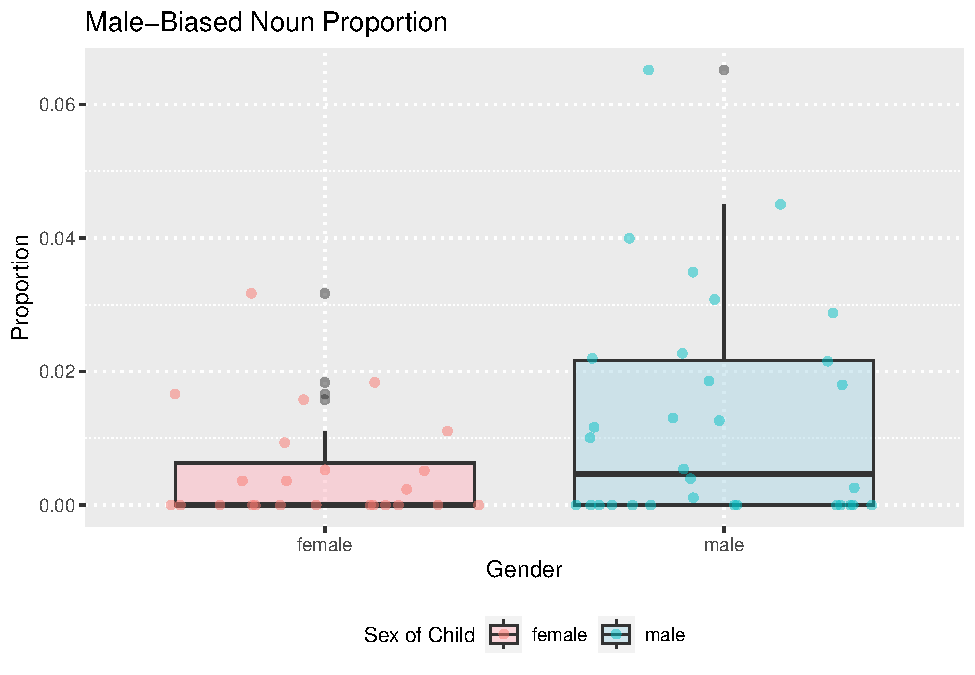
\includegraphics{My-Notebook_files/figure-latex/male-nouns-1.pdf}

X-axis: The gloss variable, representing different words (like ``dress'', ``doll'', ``necklace'', etc.). Y-axis: The count or frequency of each word, indicating how often each word appears in the dataset. Type of Plot: Bar Chart. Comparison Across Groups?: Yes Anticipated Findings: mothers speak more female-biased nouns to female infants than to male infants

As seen in Figure \ref{fig:my-figure}, There's gender bias in the nouns of mother's infant-directed speech.

\hypertarget{assignment-13.-prettified-plot}{%
\section{Assignment 13. Prettified Plot}\label{assignment-13.-prettified-plot}}

\begin{figure}
\centering
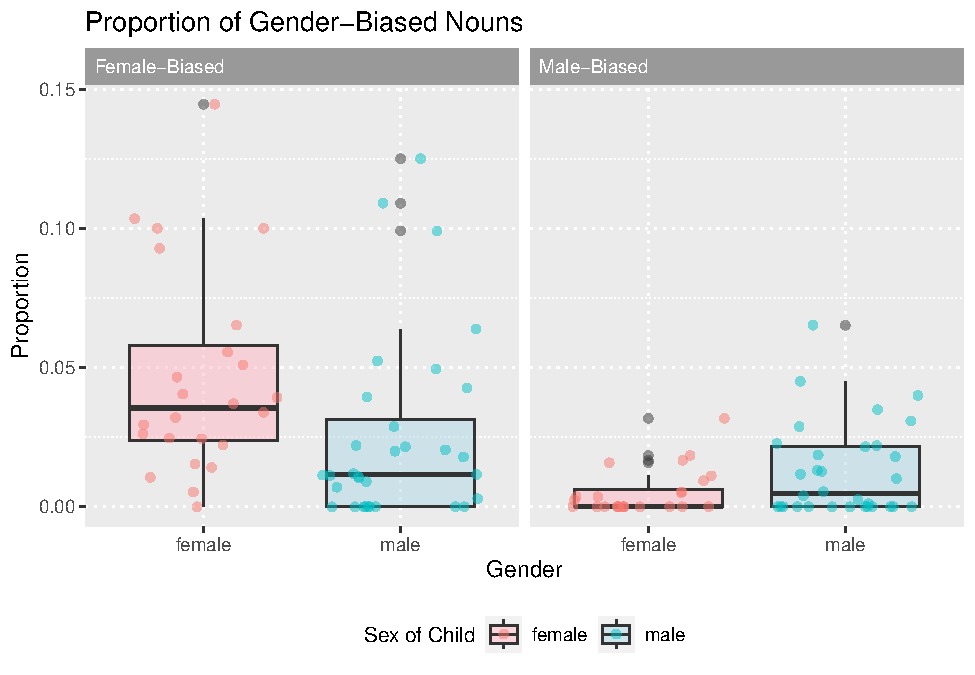
\includegraphics{My-Notebook_files/figure-latex/my-figure-1.pdf}
\caption{\label{fig:my-figure}Proportion of Gender-Biased Nouns by Gender}
\end{figure}

X-axis: female/male infants\\
Y-axis: counts of frequency of female-biased nouns Type of Plot: box plot\\
Comparison Across Groups?: Yes\\
Anticipated Findings: mothers speak more female-biased nouns in CDS to female infants than to male infants

\hypertarget{assignment-14}{%
\section{Assignment 14}\label{assignment-14}}

\begin{table}[!h]
\centering
\caption{\label{tab:my-table}Male-Infant Data}
\centering
\begin{tabular}[t]{>{}llrrrrr}
\toprule
\cellcolor[HTML]{D3D3D3}{\textbf{target\_child\_name}} & \cellcolor[HTML]{D3D3D3}{\textbf{target\_child\_sex}} & \cellcolor[HTML]{D3D3D3}{\textbf{gloss\_count}} & \cellcolor[HTML]{D3D3D3}{\textbf{fnoun\_count}} & \cellcolor[HTML]{D3D3D3}{\textbf{mnoun\_count}} & \cellcolor[HTML]{D3D3D3}{\textbf{mnoun\_proportion}} & \cellcolor[HTML]{D3D3D3}{\textbf{fnoun\_proportion}}\\
\midrule
\textcolor{blue}{\textbf{\cellcolor{gray!10}{Aaron}}} & \cellcolor{gray!10}{male} & \cellcolor{gray!10}{57} & \cellcolor{gray!10}{0} & \cellcolor{gray!10}{0} & \cellcolor{gray!10}{0.0000000} & \cellcolor{gray!10}{0.0000000}\\
\textcolor{blue}{\textbf{Adam}} & male & 201 & 4 & 0 & 0.0000000 & 0.0199005\\
\textcolor{blue}{\textbf{\cellcolor{gray!10}{Alex}}} & \cellcolor{gray!10}{male} & \cellcolor{gray!10}{19296} & \cellcolor{gray!10}{135} & \cellcolor{gray!10}{225} & \cellcolor{gray!10}{0.0116604} & \cellcolor{gray!10}{0.0069963}\\
\textcolor{blue}{\textbf{Alfred}} & male & 91 & 2 & 2 & 0.0219780 & 0.0219780\\
\textcolor{blue}{\textbf{\cellcolor{gray!10}{Alice}}} & \cellcolor{gray!10}{female} & \cellcolor{gray!10}{2081} & \cellcolor{gray!10}{106} & \cellcolor{gray!10}{66} & \cellcolor{gray!10}{0.0317155} & \cellcolor{gray!10}{0.0509370}\\
\addlinespace
\textcolor{blue}{\textbf{Allen}} & male & 108 & 0 & 0 & 0.0000000 & 0.0000000\\
\textcolor{blue}{\textbf{\cellcolor{gray!10}{Anthony}}} & \cellcolor{gray!10}{male} & \cellcolor{gray!10}{39} & \cellcolor{gray!10}{0} & \cellcolor{gray!10}{0} & \cellcolor{gray!10}{0.0000000} & \cellcolor{gray!10}{0.0000000}\\
\textcolor{blue}{\textbf{Benjamin}} & male & 914 & 36 & 1 & 0.0010941 & 0.0393873\\
\textcolor{blue}{\textbf{\cellcolor{gray!10}{Brian}}} & \cellcolor{gray!10}{male} & \cellcolor{gray!10}{89} & \cellcolor{gray!10}{1} & \cellcolor{gray!10}{0} & \cellcolor{gray!10}{0.0000000} & \cellcolor{gray!10}{0.0112360}\\
\textcolor{blue}{\textbf{Brooke}} & female & 97 & 9 & 0 & 0.0000000 & 0.0927835\\
\addlinespace
\textcolor{blue}{\textbf{\cellcolor{gray!10}{Carol}}} & \cellcolor{gray!10}{female} & \cellcolor{gray!10}{83} & \cellcolor{gray!10}{12} & \cellcolor{gray!10}{0} & \cellcolor{gray!10}{0.0000000} & \cellcolor{gray!10}{0.1445783}\\
\textcolor{blue}{\textbf{Danielle}} & female & 90 & 5 & 0 & 0.0000000 & 0.0555556\\
\textcolor{blue}{\textbf{\cellcolor{gray!10}{David}}} & \cellcolor{gray!10}{male} & \cellcolor{gray!10}{688} & \cellcolor{gray!10}{75} & \cellcolor{gray!10}{24} & \cellcolor{gray!10}{0.0348837} & \cellcolor{gray!10}{0.1090116}\\
\textcolor{blue}{\textbf{Doug}} & male & 88 & 1 & 2 & 0.0227273 & 0.0113636\\
\textcolor{blue}{\textbf{\cellcolor{gray!10}{Emily}}} & \cellcolor{gray!10}{female} & \cellcolor{gray!10}{142} & \cellcolor{gray!10}{2} & \cellcolor{gray!10}{0} & \cellcolor{gray!10}{0.0000000} & \cellcolor{gray!10}{0.0140845}\\
\addlinespace
\textcolor{blue}{\textbf{Emma}} & female & 180 & 4 & 3 & 0.0166667 & 0.0222222\\
\textcolor{blue}{\textbf{\cellcolor{gray!10}{Erica}}} & \cellcolor{gray!10}{female} & \cellcolor{gray!10}{123} & \cellcolor{gray!10}{3} & \cellcolor{gray!10}{0} & \cellcolor{gray!10}{0.0000000} & \cellcolor{gray!10}{0.0243902}\\
\textcolor{blue}{\textbf{Ethan}} & male & 23210 & 269 & 715 & 0.0308057 & 0.0115898\\
\textcolor{blue}{\textbf{\cellcolor{gray!10}{Jarret}}} & \cellcolor{gray!10}{male} & \cellcolor{gray!10}{99} & \cellcolor{gray!10}{0} & \cellcolor{gray!10}{1} & \cellcolor{gray!10}{0.0101010} & \cellcolor{gray!10}{0.0000000}\\
\textcolor{blue}{\textbf{Jas}} & male & 185 & 2 & 1 & 0.0054054 & 0.0108108\\
\addlinespace
\textcolor{blue}{\textbf{\cellcolor{gray!10}{Jase}}} & \cellcolor{gray!10}{male} & \cellcolor{gray!10}{1777} & \cellcolor{gray!10}{88} & \cellcolor{gray!10}{71} & \cellcolor{gray!10}{0.0399550} & \cellcolor{gray!10}{0.0495217}\\
\textcolor{blue}{\textbf{Jeff}} & male & 88 & 0 & 0 & 0.0000000 & 0.0000000\\
\textcolor{blue}{\textbf{\cellcolor{gray!10}{Jessica}}} & \cellcolor{gray!10}{female} & \cellcolor{gray!10}{120} & \cellcolor{gray!10}{12} & \cellcolor{gray!10}{0} & \cellcolor{gray!10}{0.0000000} & \cellcolor{gray!10}{0.1000000}\\
\textcolor{blue}{\textbf{Jillian}} & female & 2550 & 75 & 6 & 0.0023529 & 0.0294118\\
\textcolor{blue}{\textbf{\cellcolor{gray!10}{Johnnie}}} & \cellcolor{gray!10}{male} & \cellcolor{gray!10}{222} & \cellcolor{gray!10}{22} & \cellcolor{gray!10}{10} & \cellcolor{gray!10}{0.0450450} & \cellcolor{gray!10}{0.0990991}\\
\addlinespace
\textcolor{blue}{\textbf{Katie}} & female & 81 & 3 & 0 & 0.0000000 & 0.0370370\\
\textcolor{blue}{\textbf{\cellcolor{gray!10}{Kevin}}} & \cellcolor{gray!10}{male} & \cellcolor{gray!10}{139} & \cellcolor{gray!10}{4} & \cellcolor{gray!10}{4} & \cellcolor{gray!10}{0.0287770} & \cellcolor{gray!10}{0.0287770}\\
\textcolor{blue}{\textbf{Kimberly}} & female & 86 & 4 & 0 & 0.0000000 & 0.0465116\\
\textcolor{blue}{\textbf{\cellcolor{gray!10}{Laura}}} & \cellcolor{gray!10}{female} & \cellcolor{gray!10}{1360} & \cellcolor{gray!10}{55} & \cellcolor{gray!10}{25} & \cellcolor{gray!10}{0.0183824} & \cellcolor{gray!10}{0.0404412}\\
\textcolor{blue}{\textbf{Laura\_Aurie}} & female & 4 & 0 & 0 & 0.0000000 & 0.0000000\\
\addlinespace
\textcolor{blue}{\textbf{\cellcolor{gray!10}{Laurel}}} & \cellcolor{gray!10}{female} & \cellcolor{gray!10}{276} & \cellcolor{gray!10}{18} & \cellcolor{gray!10}{1} & \cellcolor{gray!10}{0.0036232} & \cellcolor{gray!10}{0.0652174}\\
\textcolor{blue}{\textbf{Lily}} & female & 38035 & 1289 & 356 & 0.0093598 & 0.0338898\\
\textcolor{blue}{\textbf{\cellcolor{gray!10}{Martin}}} & \cellcolor{gray!10}{male} & \cellcolor{gray!10}{773} & \cellcolor{gray!10}{33} & \cellcolor{gray!10}{2} & \cellcolor{gray!10}{0.0025873} & \cellcolor{gray!10}{0.0426908}\\
\textcolor{blue}{\textbf{Matt}} & male & 3947 & 85 & 50 & 0.0126678 & 0.0215353\\
\textcolor{blue}{\textbf{\cellcolor{gray!10}{Matthew}}} & \cellcolor{gray!10}{male} & \cellcolor{gray!10}{49} & \cellcolor{gray!10}{0} & \cellcolor{gray!10}{0} & \cellcolor{gray!10}{0.0000000} & \cellcolor{gray!10}{0.0000000}\\
\addlinespace
\textcolor{blue}{\textbf{Megan}} & female & 190 & 2 & 3 & 0.0157895 & 0.0105263\\
\textcolor{blue}{\textbf{\cellcolor{gray!10}{Naima}}} & \cellcolor{gray!10}{female} & \cellcolor{gray!10}{36986} & \cellcolor{gray!10}{964} & \cellcolor{gray!10}{410} & \cellcolor{gray!10}{0.0110853} & \cellcolor{gray!10}{0.0260639}\\
\textcolor{blue}{\textbf{Nanette}} & female & 609 & 15 & 0 & 0.0000000 & 0.0246305\\
\textcolor{blue}{\textbf{\cellcolor{gray!10}{Nicole}}} & \cellcolor{gray!10}{female} & \cellcolor{gray!10}{100} & \cellcolor{gray!10}{10} & \cellcolor{gray!10}{0} & \cellcolor{gray!10}{0.0000000} & \cellcolor{gray!10}{0.1000000}\\
\textcolor{blue}{\textbf{Patricia}} & female & 567 & 3 & 3 & 0.0052910 & 0.0052910\\
\addlinespace
\textcolor{blue}{\textbf{\cellcolor{gray!10}{Patrick}}} & \cellcolor{gray!10}{male} & \cellcolor{gray!10}{8} & \cellcolor{gray!10}{1} & \cellcolor{gray!10}{0} & \cellcolor{gray!10}{0.0000000} & \cellcolor{gray!10}{0.1250000}\\
\textcolor{blue}{\textbf{Peter}} & male & 49 & 1 & 0 & 0.0000000 & 0.0204082\\
\textcolor{blue}{\textbf{\cellcolor{gray!10}{Richard}}} & \cellcolor{gray!10}{male} & \cellcolor{gray!10}{345} & \cellcolor{gray!10}{1} & \cellcolor{gray!10}{0} & \cellcolor{gray!10}{0.0000000} & \cellcolor{gray!10}{0.0028986}\\
\textcolor{blue}{\textbf{Rick}} & male & 974 & 51 & 21 & 0.0215606 & 0.0523614\\
\textcolor{blue}{\textbf{\cellcolor{gray!10}{Robert}}} & \cellcolor{gray!10}{male} & \cellcolor{gray!10}{56} & \cellcolor{gray!10}{1} & \cellcolor{gray!10}{0} & \cellcolor{gray!10}{0.0000000} & \cellcolor{gray!10}{0.0178571}\\
\addlinespace
\textcolor{blue}{\textbf{Roman}} & male & 111 & 1 & 2 & 0.0180180 & 0.0090090\\
\textcolor{blue}{\textbf{\cellcolor{gray!10}{Ronny}}} & \cellcolor{gray!10}{male} & \cellcolor{gray!10}{721} & \cellcolor{gray!10}{46} & \cellcolor{gray!10}{47} & \cellcolor{gray!10}{0.0651872} & \cellcolor{gray!10}{0.0638003}\\
\textcolor{blue}{\textbf{Sarah}} & female & 51 & 2 & 0 & 0.0000000 & 0.0392157\\
\textcolor{blue}{\textbf{\cellcolor{gray!10}{Scott}}} & \cellcolor{gray!10}{male} & \cellcolor{gray!10}{91} & \cellcolor{gray!10}{0} & \cellcolor{gray!10}{0} & \cellcolor{gray!10}{0.0000000} & \cellcolor{gray!10}{0.0000000}\\
\textcolor{blue}{\textbf{Shawna}} & female & 29 & 3 & 0 & 0.0000000 & 0.1034483\\
\addlinespace
\textcolor{blue}{\textbf{\cellcolor{gray!10}{Stephen}}} & \cellcolor{gray!10}{male} & \cellcolor{gray!10}{153} & \cellcolor{gray!10}{0} & \cellcolor{gray!10}{2} & \cellcolor{gray!10}{0.0130719} & \cellcolor{gray!10}{0.0000000}\\
\textcolor{blue}{\textbf{Tommy}} & male & 83 & 0 & 0 & 0.0000000 & 0.0000000\\
\textcolor{blue}{\textbf{\cellcolor{gray!10}{Victor}}} & \cellcolor{gray!10}{male} & \cellcolor{gray!10}{504} & \cellcolor{gray!10}{6} & \cellcolor{gray!10}{2} & \cellcolor{gray!10}{0.0039683} & \cellcolor{gray!10}{0.0119048}\\
\textcolor{blue}{\textbf{Violet}} & female & 14361 & 460 & 52 & 0.0036209 & 0.0320312\\
\textcolor{blue}{\textbf{\cellcolor{gray!10}{Wendy}}} & \cellcolor{gray!10}{female} & \cellcolor{gray!10}{195} & \cellcolor{gray!10}{3} & \cellcolor{gray!10}{1} & \cellcolor{gray!10}{0.0051282} & \cellcolor{gray!10}{0.0153846}\\
\addlinespace
\textcolor{blue}{\textbf{William}} & male & 15388 & 160 & 286 & 0.0185859 & 0.0103977\\
\bottomrule
\end{tabular}
\end{table}

As shown in Table \ref{tab:my-table}, the gender distribution in the dataset varies, with a higher percentage of Female compared to Male.

\hypertarget{assignment-15-16}{%
\section{Assignment 15 \& 16}\label{assignment-15-16}}

\hypertarget{descriptive-analysis-examining-maternal-gender-biased-language-imput-patterns}{%
\subsection{\texorpdfstring{\emph{Descriptive Analysis}: Examining Maternal Gender-Biased Language Imput Patterns}{Descriptive Analysis: Examining Maternal Gender-Biased Language Imput Patterns}}\label{descriptive-analysis-examining-maternal-gender-biased-language-imput-patterns}}

\begin{verbatim}
## # A tibble: 2 x 4
##   target_child_sex mean_mnoun median_mnoun sd_mnoun
##   <chr>                 <dbl>        <dbl>    <dbl>
## 1 female              0.00513      0        0.00817
## 2 male                0.0128       0.00469  0.0165
\end{verbatim}

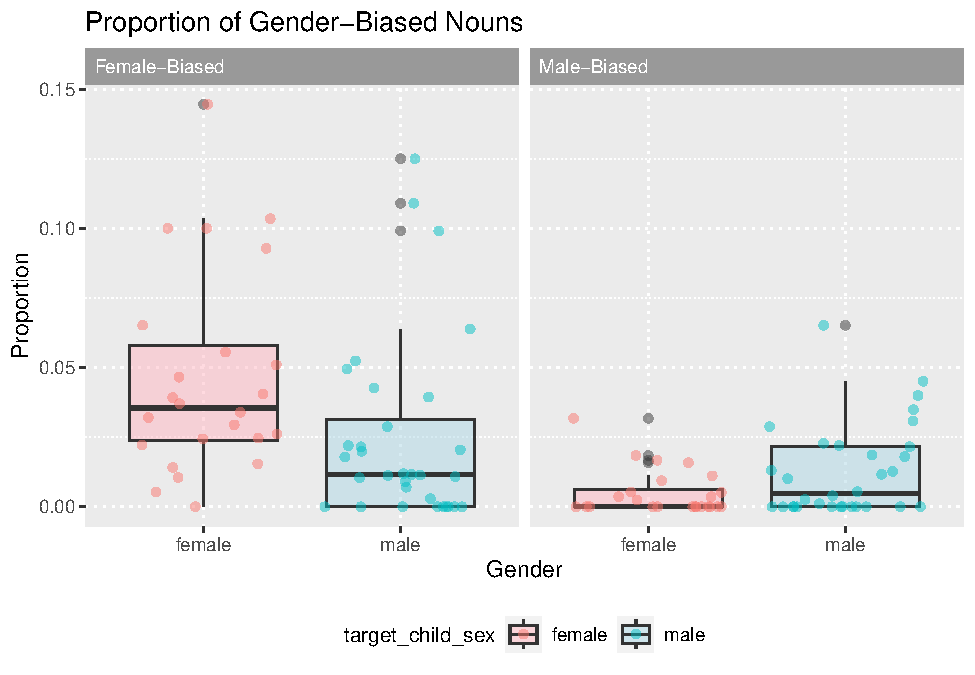
\includegraphics{My-Notebook_files/figure-latex/descriptive-analysis-1.pdf}

\hypertarget{hypothesis-testing-analysis-testing-the-influence-of-childs-gender-on-maternal-language-input}{%
\subsection{\texorpdfstring{\emph{Hypothesis Testing Analysis}: Testing the Influence of Child's Gender on Maternal Language Input}{Hypothesis Testing Analysis: Testing the Influence of Child's Gender on Maternal Language Input}}\label{hypothesis-testing-analysis-testing-the-influence-of-childs-gender-on-maternal-language-input}}

\begin{verbatim}
##                  Df   Sum Sq   Mean Sq F value Pr(>F)  
## target_child_sex  1 0.000798 0.0007977   4.326 0.0423 *
## Residuals        54 0.009958 0.0001844                 
## ---
## Signif. codes:  0 '***' 0.001 '**' 0.01 '*' 0.05 '.' 0.1 ' ' 1
\end{verbatim}

\begin{verbatim}
##                  Df  Sum Sq  Mean Sq F value Pr(>F)  
## target_child_sex  1 0.00633 0.006327   5.252 0.0259 *
## Residuals        54 0.06506 0.001205                 
## ---
## Signif. codes:  0 '***' 0.001 '**' 0.01 '*' 0.05 '.' 0.1 ' ' 1
\end{verbatim}

\hypertarget{assignment-17}{%
\section{Assignment 17}\label{assignment-17}}

The ANOVA tests conducted on the proportions of female-biased nouns used by mothers reveal the following:
The Tukey test results are:

\begin{table}

\caption{\label{tab:unnamed-chunk-9}Tukey HSD Test Results for Target Child Sex}
\centering
\begin{tabular}[t]{l|r|r|r|r}
\hline
  & diff & lwr & upr & p adj\\
\hline
male-female & -0.0214792 & -0.0402707 & -0.0026877 & 0.0258534\\
\hline
\end{tabular}
\end{table}

For female-biased nouns used by mothers, the F-statistic is \(F\) = 5.25, \(p\) = 0.03.

And for male-biased nouns used by mothers, the F-statistic is \(F\) = 4.33, \(p\) = 0.04.

The results suggest that there is a statistically significant difference in the usage of gender-biased nouns by mothers when speaking to male children compared to female children, at the conventional 0.05 significance level.

\newpage

\hypertarget{references}{%
\section{References}\label{references}}

\begingroup
\setlength{\parindent}{-0.5in}
\setlength{\leftskip}{0.5in}

\hypertarget{refs}{}
\begin{CSLReferences}{1}{0}
\leavevmode\vadjust pre{\hypertarget{ref-adamsGenderDifferencesParentchild1995}{}}%
Adams, S., Kuebli, J., Boyle, P. A., \& Fivush, R. (1995). Gender differences in parent-child conversations about past emotions: {A} longitudinal investigation. \emph{Sex Roles}, \emph{33}(5-6), 309--323. \url{https://doi.org/10.1007/BF01954572}

\leavevmode\vadjust pre{\hypertarget{ref-birnsEmergenceSocializationSex1976}{}}%
Birns, B. (1976). The {Emergence} and {Socialization} of {Sex Differences} in the {Earliest Years}. \emph{Merrill-Palmer Quarterly of Behavior and Development}, \emph{22}(3), 229--254. Retrieved from \url{https://www.jstor.org/stable/23084603}

\leavevmode\vadjust pre{\hypertarget{ref-crowleySharedScientificThinking2001}{}}%
Crowley, K., Callanan, M. A., Jipson, J. L., Galco, J., Topping, K., \& Shrager, J. (2001). Shared scientific thinking in everyday parent-child activity. \emph{Science Education}, \emph{85}(6), 712--732. \url{https://doi.org/10.1002/sce.1035}

\leavevmode\vadjust pre{\hypertarget{ref-ecclesGenderRoleStereotypes1990}{}}%
Eccles, J. S., Jacobs, J. E., \& Harold, R. D. (1990). Gender {Role Stereotypes}, {Expectancy Effects}, and {Parents}' {Socialization} of {Gender Differences}. \emph{Journal of Social Issues}, \emph{46}(2), 183--201. \url{https://doi.org/10.1111/j.1540-4560.1990.tb01929.x}

\leavevmode\vadjust pre{\hypertarget{ref-ferjanramirezFathersInfantdirectedSpeech2022}{}}%
Ferjan Ramírez, N. (2022). Fathers' infant-directed speech and its effects on child language development. \emph{Language and Linguistics Compass}, \emph{16}(1), e12448. \url{https://doi.org/10.1111/lnc3.12448}

\leavevmode\vadjust pre{\hypertarget{ref-honigSexRoleSocialization1983}{}}%
Honig, A. S. (1983). Sex {Role Socialization} in {Early Childhood}. \emph{Young Children}, \emph{38}(6), 57--70. Retrieved from \url{https://www.jstor.org/stable/42643128}

\leavevmode\vadjust pre{\hypertarget{ref-kachergisEstimatingDemographicBias2023}{}}%
Kachergis, G., Francis, N., \& Frank, M. C. (2023). Estimating {Demographic Bias} on {Tests} of {Children}'s {Early Vocabulary}. \emph{Topics in Cognitive Science}, \emph{15}(2), 303--314. \url{https://doi.org/10.1111/tops.12635}

\leavevmode\vadjust pre{\hypertarget{ref-wallentinCrossCulturalSexGender2023}{}}%
Wallentin, M., \& Trecca, F. (2023). Cross-{Cultural Sex}/{Gender Differences} in {Produced Word Content Before} the {Age} of 3 {Years}. \emph{Psychological Science}, \emph{34}(4), 411--423. \url{https://doi.org/10.1177/09567976221146537}

\leavevmode\vadjust pre{\hypertarget{ref-weitzmanTraditionalNontraditionalMothers1985}{}}%
Weitzman, N., Birns, B., \& Friend, R. (1985). Traditional and {Nontraditional Mothers}' {Communication} with {Their Daughters} and {Sons}. \emph{Child Development}, \emph{56}(4), 894--898. \url{https://doi.org/10.2307/1130101}

\end{CSLReferences}

\endgroup


\end{document}
